\documentclass{scrartcl}

\usepackage{hyperref}
\usepackage{graphicx}

\begin{document}

\title{Gradr: Scalable Automatic Grading for Everyone}
\subtitle{System Overview, Load Testing, and Experience Report}
\author{Kyle Dewey, Jared Roesch, and Daniel Spokoyny}
\date{December 15, 2014}

\maketitle

\section{Introduction}
Gradr is a cloud-based system for automatically building, testing, and grading student solutions to class assignments.
The ultimate end goal of Gradr is to be used in MOOC-like settings, where it acts as a student submission system, an automated feedback generator, and an automated grader.

The goals of Gradr bring up a number of technical challenges relating to scalability.
Not only do the number of submissions become large in this setting, erratic usage patterns are a problem (e.g., many submissions just before a deadline).
For this reason, Gradr must be designed in a way which is not only scalable (for the overall load), but elastic --- we should be able to dynamically add and remove system resources as needed.

\section{System Overview}
Gradr is implemented as a distributed system with multiple components, which allows for concerns to be separated out and for horizontal scaling to be inserted at key points.
Where possible, we have used components from elsewhere which satisfy our needs.
A description of the different components in Gradr follows:

\begin{description}
  \item[GitHub~\cite{github}] \hfill \\
    A publicly-available hosting service for code repositories, focused around the \texttt{git}~\cite{git} revision control system.
    GitHub stores student solutions, lifting the burden of code storage off of Gradr.
    GitHub also informs the rest of the Gradr system whenever code is submitted (via a typical \texttt{push}), triggering downstream building to occur.

  \item[Postgres~\cite{postgres}] \hfill \\
    A popular relational database engine, which serves to store persistent information.
    Postgres also facilitates communication between different components of Gradr, as it stores globally synchronized state.

  \item[Notification Listener] \hfill \\
    A custom component which listens for \texttt{push} notifications from GitHub via a webhook~\cite{github_webhook}.
    Whenever a student performs a \texttt{push}, GitHub performs a standard \texttt{POST} request to this service, providing:
    \begin{itemize}
      \item The unique GitHub username of the student performing the \texttt{push} (which is ultimately mapped back to a unique username in Gradr)
      \item The name of the repository the student \texttt{push}ed to (which is ultimately mapped back to a unique assignment identifier in Gradr)
      \item The branch on which the \texttt{push} occurred
    \end{itemize}
    The above information is put into the Postgres database, and is marked as pending for downstream processing.

  \item[Worker] \hfill \\
    A custom component which regularly polls the Postgres database, looking for student submissions which are marked as pending.
    The worker will first select a pending entry, and mark it as being processed.
    The worker will then download the submission from GitHub, compile it, run tests, and put the test results pack into the Postgres database, finally marking the entry as complete.
    Crucial to Gradr's design is the fact that there can exist any number of worker components at any time.

  \item[Frontend] \hfill \\
    A custom web application which students and instructors can use to view feedback on their submissions, which was derived from workers.
    Much like workers, there can exist multiple frontend components at any time.
\end{description}

A graphical representation of these components, along with the data flow between them, can be seen in Figure~\ref{fig:system_overview}.

\begin{figure}[here]
  \begin{center}
    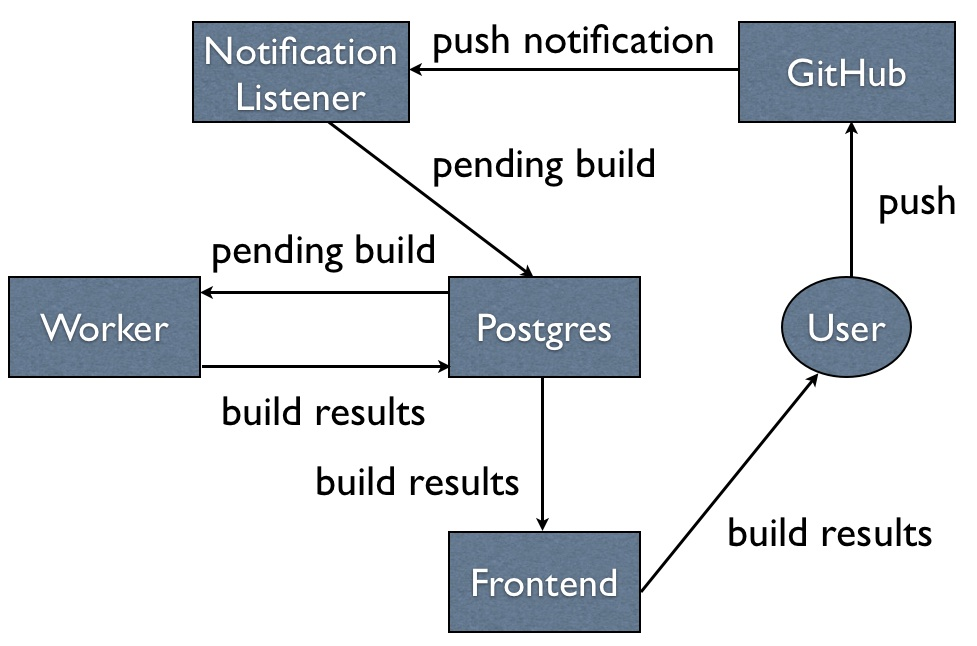
\includegraphics[scale=0.45]{non_graph_images/system_overview.jpg}
  \end{center}
  \caption{Diagram of overall Gradr architecture, along with data flow between components and the user}
  \label{fig:system_overview}
\end{figure}

\section{Load Testing}
\subsection{Critical Paths}
With respect to how Gradr is intended to be used, we identify three critical paths:

\begin{itemize}
  \item The process of polling pending builds from the database and putting results into the database
  \item The process of putting a pending build into the database from a GitHub \texttt{push} notification
  \item Users viewing build results on the frontend
\end{itemize}

The rest of the report focuses on the first of these tasks, as it is expected to be the most executed part of the architecture.

\subsection{Experimental Setup}
For all experimenents, we used RDS~\cite{rds} with a single \texttt{db.ts.small} instance.
As we focus only on builds, the number of notification listeners and frontend systems was kept constant at one.

Submitted code was carefully controlled, and kept uniform for the duration of individual experiments.
The actual submitted code can be found at \url{https://github.com/kyledewey/test-gradr}.
Two student submissions were used, described below:
\begin{description}
  \item[\texttt{sleephalf}] \hfill \\
    Under the \texttt{sleephalf} branch, the code when run will sleep for a half of a second, and then print out some fake test results.

  \item[\texttt{sleep3}] \hfill \\
    Under the \texttt{sleep3} branch, the code when run will sleep for a three seconds, and then print out some fake test results.
\end{description}

The reason why both submissions simply sleep as opposed to doing a real code build and test cycle is because this cuts out large amount of variability between individual instances.
We can know for sure that the build should take a precise, fixed amount of time under all circumstances.
This allows us to focus in on communication overhead within the system and other related issues.
While this unit time property is unrealistic, in practice, issues pertaining to CPU or IO-intensive builds could be simply adjusted by using bigger instance types, and these are not issues fundamental to Gradr itself.

Workers were distributed in five different ways, described below:
\begin{description}
  \item[Single Small] \hfill \\
    A single worker process runs on a single \texttt{t2.small} EC2~\cite{ec2} instance.

  \item[Two Small] \hfill \\
    Each of two \texttt{t2.small} EC2 instances run a single worker process.

  \item[Four Small] \hfill \\
    Each of four \texttt{t2.small} EC2 instances run a single worker process.

  \item[One Large] \hfill \\
    Two worker processes run on a single \texttt{m3.large} EC2 instance.

  \item[Two Large] \hfill \\
    Each of two \texttt{m3.large} EC2 instances run two worker processes.
\end{description}

For all experiments, we sent 100 push notifications of whichever chosen repository and branch to the notification listener, initially with no running workers.
Once all notifications were sent, workers were started in parallel in the formation according to whichever AWS configuration was chosen.
While experiments are running, we measure the number of pending builds (queue length) over time.
Once an experiment finishes, we determine the average amount of time each build took, starting from the point where a build was selected for processing and ending with the time the results were posted.

The goal with measuring the queue length over time is to identify any anomalies in communication.
We would expect in all cases a straight line, and any other shape would indicate issues related to predictability, such as non-constant communication overhead.

The goal with measuring the average time of each build is to determine the overall overhead of the system itself.
Since the time each build takes is known in advance, we know that any additional time is purely overhead of our system.

The goal with varying the instance configuration is to identify any sort of unseen computational and network bottlenecks, along with measuring scalability of the system.
If the worker process is CPU-intensive independent of the actual student code, then this would reveal itself as bigger instance types performing better than smaller instance types.
Additionally, in a perfectly scalable environment we would expect to see that twice as many worker threads can clear a queue of pending builds in half the time, and so on.
This would not be true of a high-contension situation, and would be strong cause to optimize.

\subsection{Results and Discussion}
We breakdown the results according to the type of the code submission used (either \texttt{sleephalf} or \texttt{sleep3}).

\subsubsection{\texttt{sleephalf}}
\label{sec:sleephalf}
Charts showing the queue length reduction over time are shown below in Figures~\ref{fig:sleephalf_one_small_queuelength}, \ref{fig:sleephalf_two_small_queuelength}, \ref{fig:sleephalf_four_small_queuelength}, \ref{fig:sleephalf_one_large_queuelength}, and~\ref{fig:sleephalf_two_large_queuelength}.

\begin{figure}[here]
  \begin{center}
    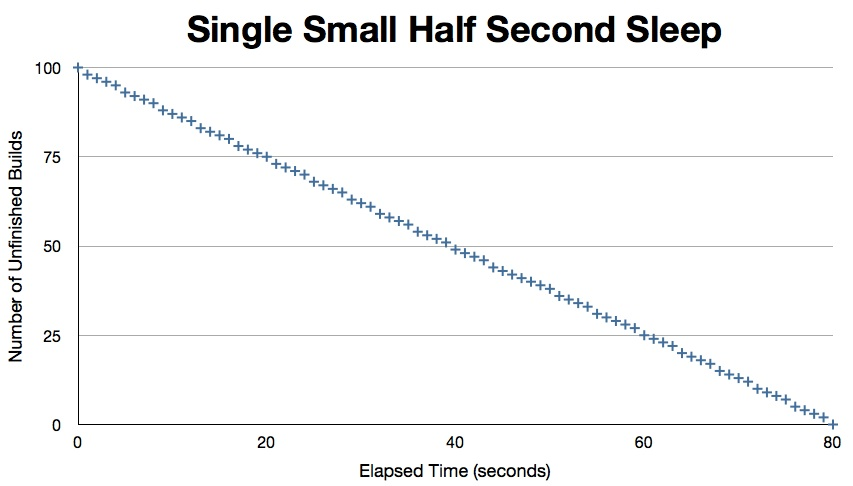
\includegraphics[scale=0.45]{raw_data/sleep0.5/one_small/graph.jpg}
  \end{center}
  \caption{Single Small Half Second Sleep}
  \label{fig:sleephalf_one_small_queuelength}
\end{figure}

\begin{figure}[here]
  \begin{center}
    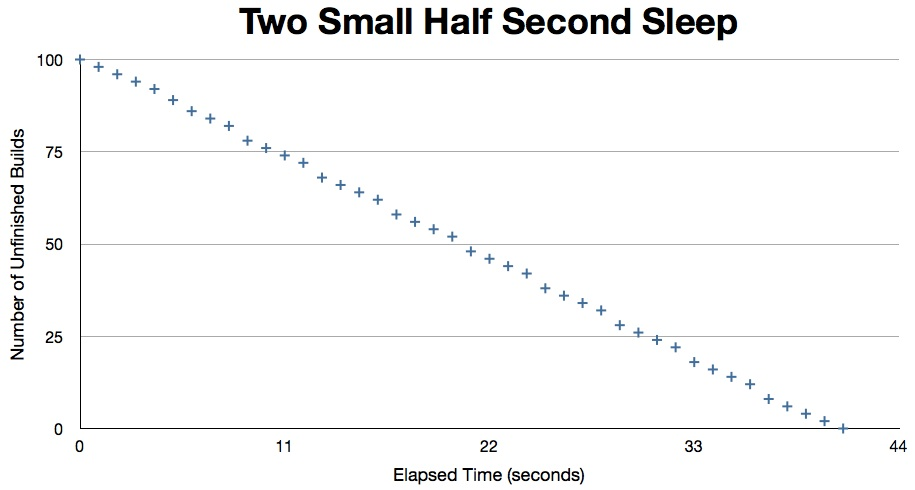
\includegraphics[scale=0.45]{raw_data/sleep0.5/two_small/graph.jpg}
  \end{center}
  \caption{Two Small Half Second Sleep}
  \label{fig:sleephalf_two_small_queuelength}
\end{figure}

\begin{figure}[here]
  \begin{center}
    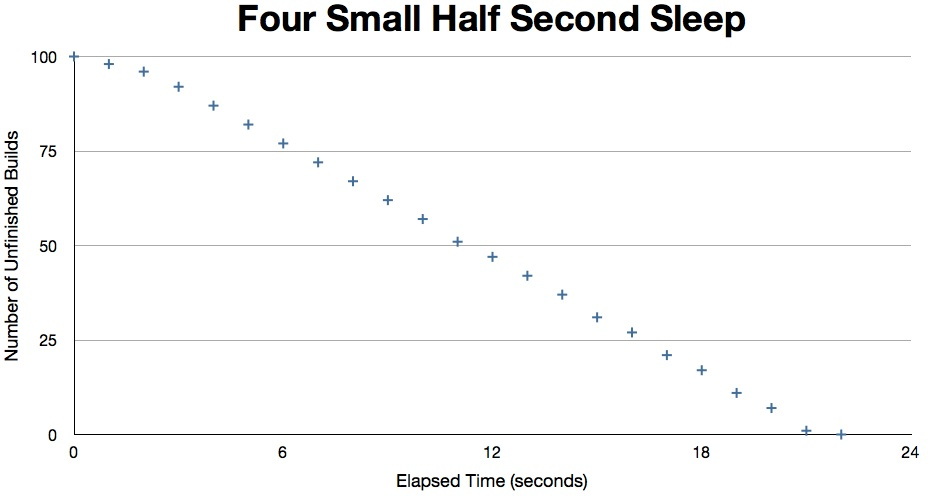
\includegraphics[scale=0.45]{raw_data/sleep0.5/four_small/graph.jpg}
  \end{center}
  \caption{Four Small Half Second Sleep}
  \label{fig:sleephalf_four_small_queuelength}
\end{figure}

\begin{figure}[here]
  \begin{center}
    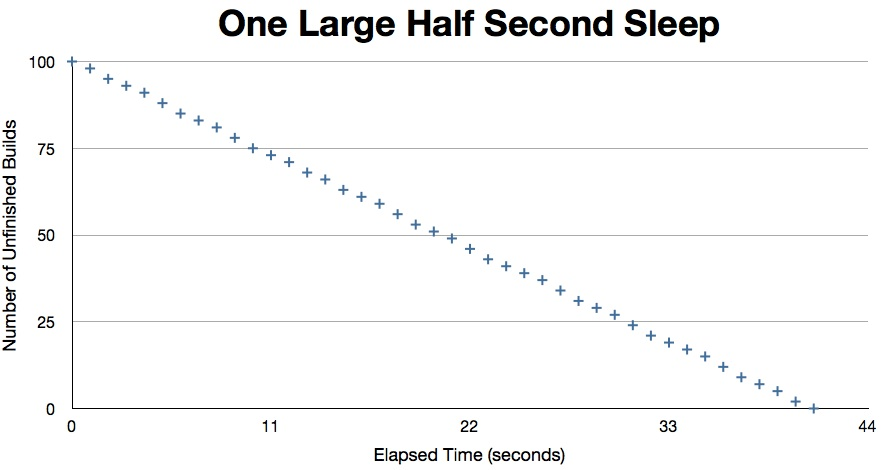
\includegraphics[scale=0.45]{raw_data/sleep0.5/one_large/graph.jpg}
  \end{center}
  \caption{One Large Half Second Sleep}
  \label{fig:sleephalf_one_large_queuelength}
\end{figure}

\begin{figure}[here]
  \begin{center}
    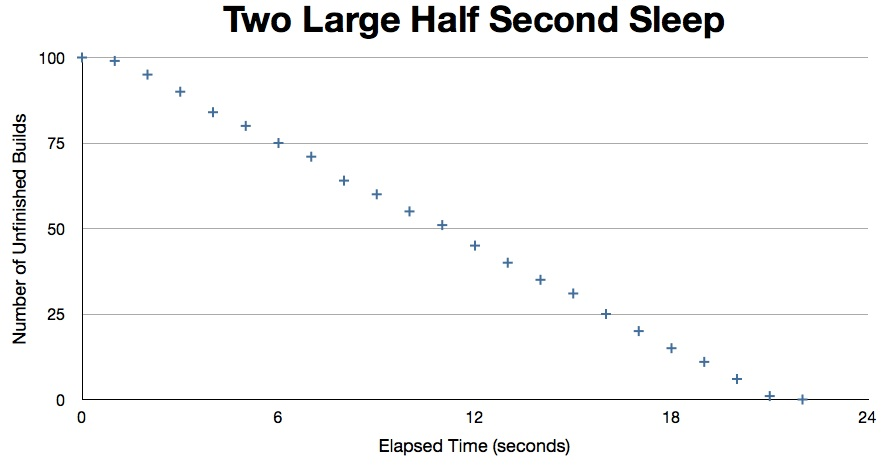
\includegraphics[scale=0.45]{raw_data/sleep0.5/two_large/graph.jpg}
  \end{center}
  \caption{Two Large Half Second Sleep}
  \label{fig:sleephalf_two_large_queuelength}
\end{figure}

As shown, in nearly all cases, the trend is a downward straight line, illustrating both that the system is predictable and communication overhead is constant.
There is a slight curve at the end of the trend in Figure~\ref{fig:sleephalf_two_large_queuelength}, which is explained by the fact that queue length results are captured with only one-second granularity and so the line likely ended sooner in reality.
The slight curve at the start of Figure~\ref{fig:sleephalf_two_large_queuelength} can be explained by the fact that workers were starting only approximately in parallel --- there were slight delays in starting occassionally.
As such, it seems likely that a subset of the workers started processing builds before all the workers started, resulting in fewer than expected builds per second.

We also measured the global amount of time taken to process all builds between the different worker configurations, shown below in Figure~\ref{fig:sleephalf_all}.

\begin{figure}[here]
  \begin{center}
    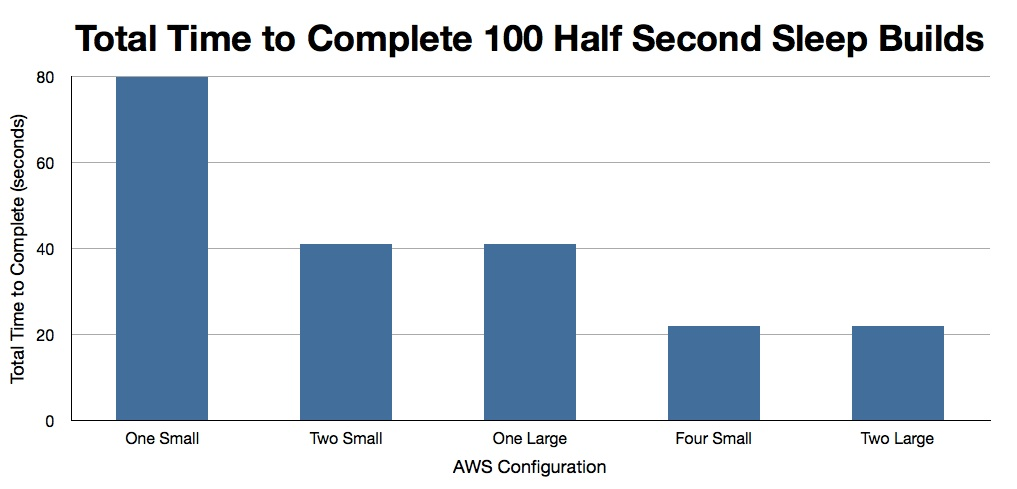
\includegraphics[scale=0.45]{raw_data/sleep0.5/time_to_complete_all.jpg}
  \end{center}
  \caption{Time to complete all builds across different worker configurations, where each build slept for half of a second}
  \label{fig:sleephalf_all}
\end{figure}

As shown, the only factor which is relevant to decreasing the amount of time taken to perform all the builds is the number of worker threads processing data.
Both the \textbf{Two Small} and \textbf{One Large} configurations take approximately the same amount of time, and similarly the \textbf{Four Small} and \textbf{Two Large} configurations, because the number of worker threads is the same --- two and four, respectively.
Additionally, the amount of time taken for \textbf{Two Small} is almost exactly half of \textbf{One Small}, and similarly the amount of time taken for \textbf{Four Small} is almost exactly half of \textbf{One Large}.
These facts indicate that we have perfect horizontal scaling of workers, at least for relatively small numbers of worker processes.

We also measured the average amount of time taken from the point when a pending build was selected from the database and the point when build results were placed in the database.
This was done for all aforementioned worker configurations.
The results are shown below in Figure~\ref{fig:sleephalf_each}.

\begin{figure}[here]
  \begin{center}
    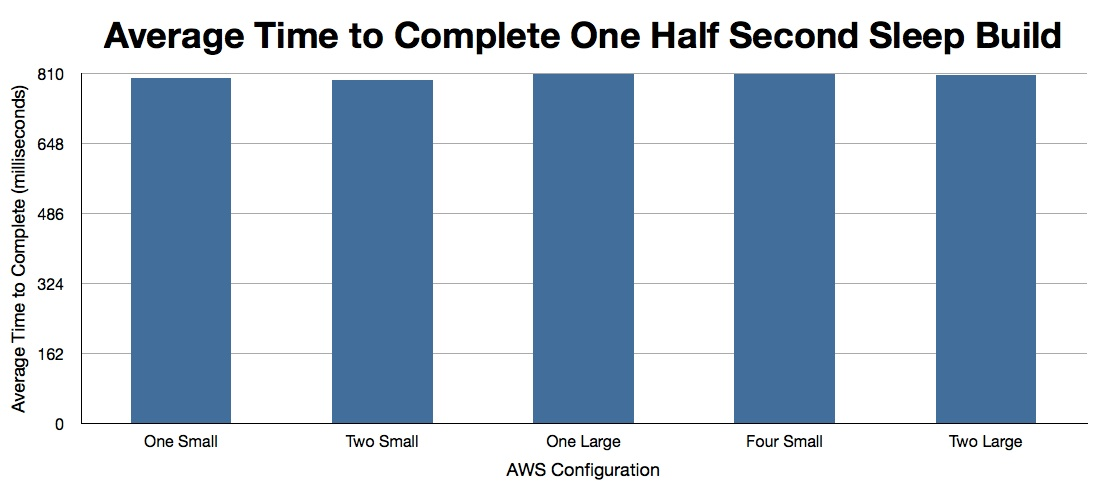
\includegraphics[scale=0.45]{raw_data/sleep0.5/time_to_complete_each.jpg}
  \end{center}
  \caption{Average time to complete a single build across different worker configurations, where each build slept for half of a second}
  \label{fig:sleephalf_each}
\end{figure}

As shown, the effect of the configuration had essentially no impact on the amount of time taken for a build, which was expected given the fact that the builds simply sleep.
Additionally, we can use this data to measure the overhead of Gradr itself.
We can see that builds take approximately 800 milliseconds.
Combining this with the fact that builds simply sleep for 500 milliseconds, we can estimate Gradr's overhead to be approximately 300 milliseconds per build.
The vast majority of this time is spent downloading code from GitHub, and was around 200 milliseconds in informal experimentation.
This shows that Gradr workers have overall very low overhead, and there is not much that can be done to improve this.

\subsubsection{\texttt{sleep3}}
\label{sec:sleep3}

Charts showing the queue length reduction over time for the \texttt{sleep3} build are shown below in Figures~\ref{fig:sleep3_one_small_queuelength}, \ref{fig:sleep3_two_small_queuelength}, \ref{fig:sleep3_four_small_queuelength}, \ref{fig:sleep3_one_large_queuelength}, and~\ref{fig:sleep3_two_large_queuelength}.

\begin{figure}[here]
  \begin{center}
    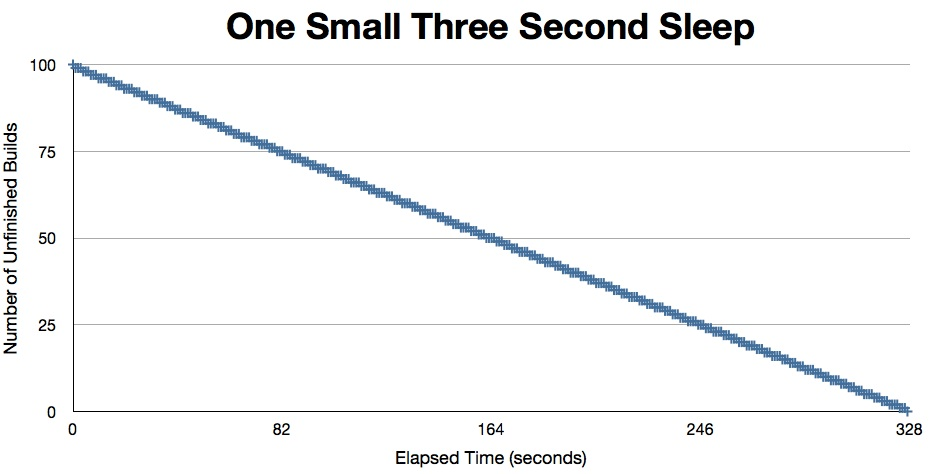
\includegraphics[scale=0.45]{raw_data/sleep3/one_small/graph.jpg}
  \end{center}
  \caption{Single Small Three Second Sleep}
  \label{fig:sleep3_one_small_queuelength}
\end{figure}

\begin{figure}[here]
  \begin{center}
    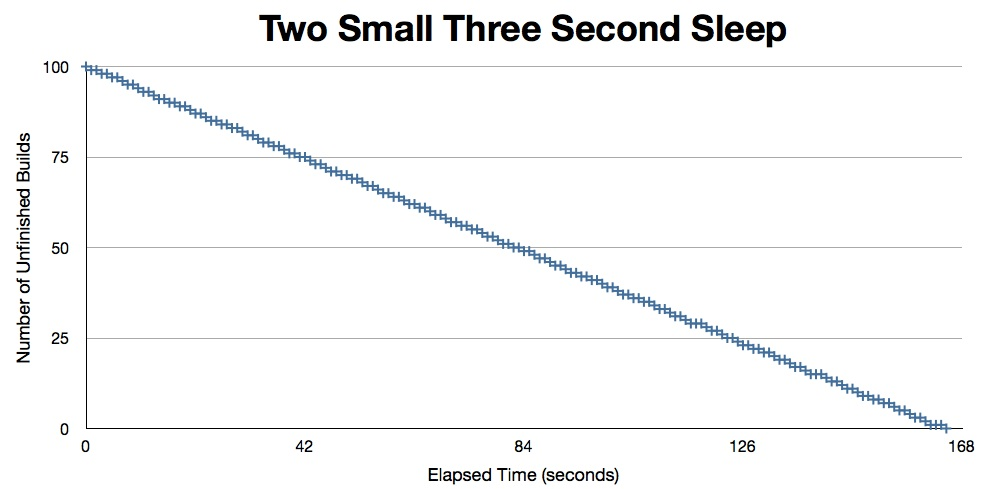
\includegraphics[scale=0.45]{raw_data/sleep3/two_small/graph.jpg}
  \end{center}
  \caption{Two Small Three Second Sleep}
  \label{fig:sleep3_two_small_queuelength}
\end{figure}

\begin{figure}[here]
  \begin{center}
    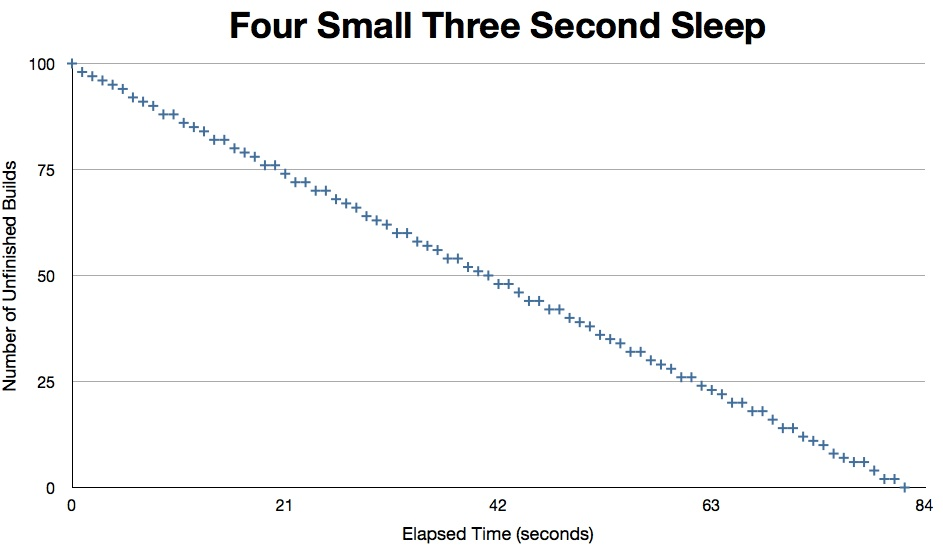
\includegraphics[scale=0.45]{raw_data/sleep3/four_small/graph.jpg}
  \end{center}
  \caption{Four Small Three Second Sleep}
  \label{fig:sleep3_four_small_queuelength}
\end{figure}

\begin{figure}[here]
  \begin{center}
    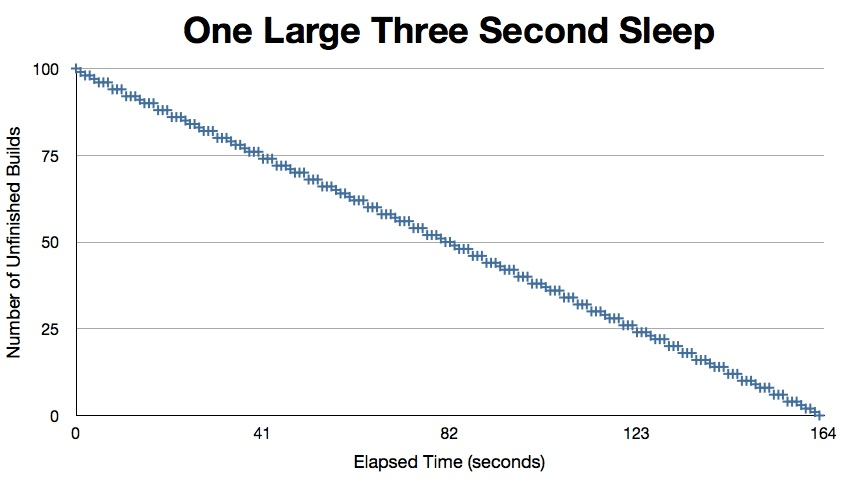
\includegraphics[scale=0.45]{raw_data/sleep3/one_large/graph.jpg}
  \end{center}
  \caption{One Large Three Second Sleep}
  \label{fig:sleep3_one_large_queuelength}
\end{figure}

\begin{figure}[here]
  \begin{center}
    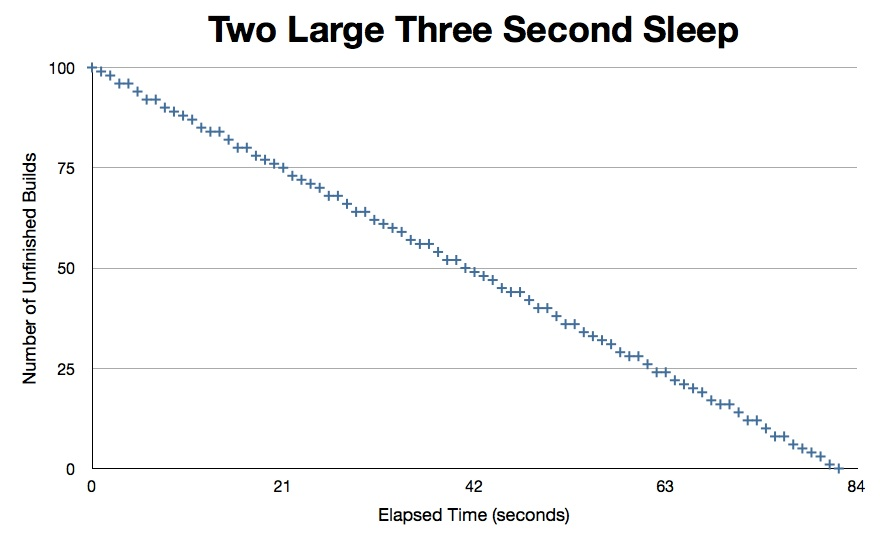
\includegraphics[scale=0.45]{raw_data/sleep3/two_large/graph.jpg}
  \end{center}
  \caption{Two Large Three Second Sleep}
  \label{fig:sleep3_two_large_queuelength}
\end{figure}

The above results are extremely similar to those of Section~\ref{sec:sleephalf}, and so we draw the same conclusions as before.

We also measured the global amount of time taken to process all builds between the different worker configurations, shown below in Figure~\ref{fig:sleep3_all}.

\begin{figure}[here]
  \begin{center}
    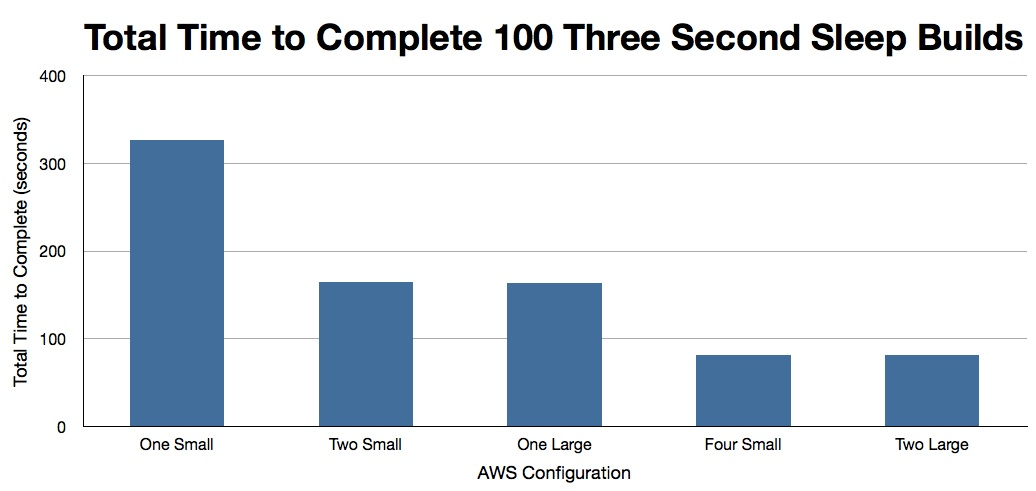
\includegraphics[scale=0.45]{raw_data/sleep3/time_to_complete_all.jpg}
  \end{center}
  \caption{Time to complete all builds across different worker configurations, where each build slept for three seconds}
  \label{fig:sleep3_all}
\end{figure}

Once again, we draw the same conclusions from Figure~\ref{fig:sleep3_all} as done in Section~\ref{sec:sleephalf}, as the shape is nearly identical.

As for the average time taken for each build, this data is shown below in Figure~\ref{fig:sleep3_each}.

\begin{figure}[here]
  \begin{center}
    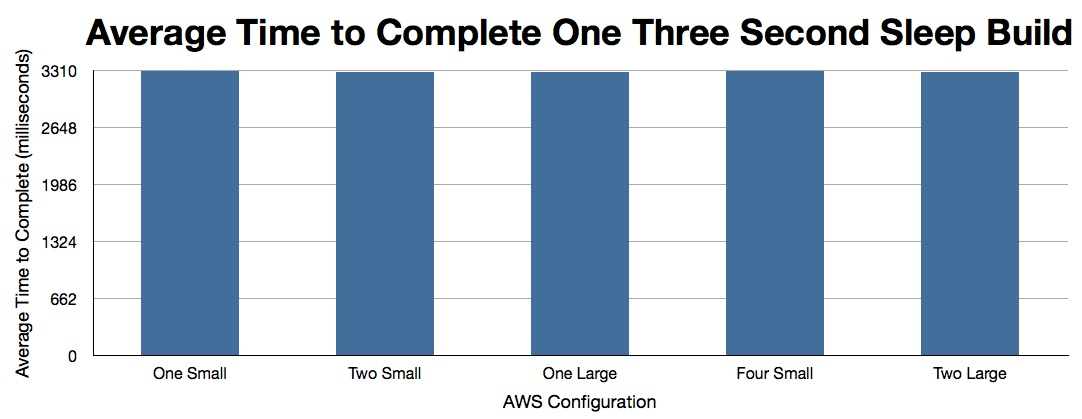
\includegraphics[scale=0.45]{raw_data/sleep3/time_to_complete_each.jpg}
  \end{center}
  \caption{Average time to complete a single build across different worker configurations, where each build slept for three seconds}
  \label{fig:sleep3_each}
\end{figure}

Once again, the total time taken did not significantly vary between the different worker configurations, leading us to conclude that there is no hidden system overhead.
The prior estimation of 300 milliseconds of system overhead also remains consistent, given that builds sleep for 3000 milliseconds (three seconds) and generally take 3300 milliseconds to complete.

Overall, we conclude that the critical path involving workers, which is likely to be the most stressed path, is both highly performant and scalable.

\subsection{Load Testing Other Critical Paths}
Some attempt was also made at stressing the path from GitHub to the notification listener.
For this experiment, 10 threads sequentially kept sending push notifications directly to the notification listener, bypassing GitHub on the assumption that GitHub may throttle back notifications.
A visible connection backlog was set to one, in an attempt to force a \texttt{POST} failure.
Even under these conditions, we were unable to get a failure to occur.
This seems to be due to two major reasons.
For one, each \texttt{POST} can be processed quite rapidly, within about 30 milliseconds including interactions with Postgres.
This time is independent of the size of the database, thanks to indecies of appropriate columns in the database.
Indeed, looking at the server, even on a \texttt{t2.small} instance the notification listener process only uses approximately 6\% of the CPU, indicating that 10 parallel senders is not enough to put sufficient strain on it.
An additional reason is that with the \texttt{HTTP} server we are using (\texttt{hyper}~\cite{hyper}), a curory glance at some of the source code hints that there may be attempts to perform parallel connections, even though this is not supposed to be case according to its documentation.
If this is true, it would take an enourmous amount of stress to start seeing failures.

As for the frontend, there has not been sufficient effort on load testing it due primarily to lack of time.
However, in Section~\ref{sec:performance_improvements}, we do discuss possible issues and solutions in this critical path.

\section{Possible Improvements}
\label{sec:performance_improvements}

\subsection{Frontend}
Put it behind a load balancer.

TODO: actually describe this.
\subsection{Backend}
\subsubsection{Notification Listener}
Make multithreaded, put behind a load balancer.

TODO: actually describe this.
\subsubsection{Worker}
If a worker fails, it can leave the system in an inconsistent state, where a submission is marked as submitted but is never built.
This can be addressed by using a fault-tolerant queue like SQS~\cite{sqs} for communication between the notification listener and workers.

TODO: actually describe this.
\subsubsection{Postgres}
Read replications.

TODO: actually describe this.

\subsubsection{Auxilliary Storage for Results}
Results can be huge, and are stored in Postgres right now for simplicity.
These could be put into an auxilliary, eventually consistent data storage if downloading results from Postgres becomes a burden.

TODO: actually describe this.

\section{On the Usage of the Rust Programming Language}
The entire backend is implemented in the Rust programming language~\cite{rust}.

\subsection{Advantages and Challenges}
\subsection{Database Operations}

\bibliography{bibtex}{}
\bibliographystyle{plain}

\end{document}
